\documentclass{article}
\usepackage[utf8]{inputenc}
\usepackage{epsfig}
\usepackage{graphicx} 
%\graphicspath{ {c:/Users/Norma Tapia/Documents/Tesis/cool} }

\title{Tesis: \ \\ Análisis de desgarres femorales. Una aplicación de Datos Circulares al campo de la medicina} %Necesito título rimbombante
\author{Por Mi :)}
\date{2016}

\begin{document}


\begin{enumerate}
	\item Introducción
	\item Descripción de los datos
	\item Análisis exploratorio y gráfico de los datos
	\item Aproximación téorica
		\begin{enumerate}
			\item Jitter
			\item ANOVA
			\item Datos circulares
		\end{enumerate}
	\item Conclusión		
\end{enumerate}

\maketitle
% ¿Cómo poner en interlineado más grande entre linea y linea?
\section{Introducción}
	Esta tesis surgió a partir de un problema real en el campo de la medicina. A continuación se describe el proyecto que dio inicio a esta investigación.

	%Esto es lo que dice el documento
	%En este proyecto había cuatro radiólogos leyendo imágenes de resonancia magnética de caderas, usando la secuencia estándar (SOC = standard of care) y una nueva llamada IDEAL. Los radiólogos evalúan el daño en el cartílago en la cabeza del fémur usando la "carátula del reloj" para descubrir su localización. A los pacientes con "labral tears" (desgarres) son operados con artroscopía, y el cirujano evalúa el daño "real". La pregunta era si IDEAL era mejor que SOC para visualizar el daño, y evaluar que tan repetibles son las lecturas entre radiólogos y las del mismo radiólogo con las dos secuencias.	
	\ \\ 
	En medicina, cuando una persona sufre un desgarre en el cartílago ubicado en la cabeza del fémur (labral tear), para conocer la localización puntual y extensión de la herida, se usa un método llamado "carátula del reloj", en el cual se dan las "coordenadas" del desgarre como si se diera la hora en un reloj de manecillas. Esto se puede apreciar por medio de una resonancia magnética. Al ser un paciente diagnosticado con desgarre, es operado por artroscopía, y el cirujano evalúa el daño real. 
	\ \\ \ \\
	Para diagnosticar, los médicos (radiólogos) tienen dos métodos: 
	\begin{enumerate}
		\item Secuencia estándar, o SOC por sus siglas en inglés (Standard of Care)
		\item Un nuevo método conocido como IDEAL % ¿qué significa IDEAL? son siglas o solo es ideal?
	\end{enumerate}	
	\ \\ 
	% Se cuenta con la información de cuatro médicos con sus correspondientes diagnósticos por ambos métodos, y el diagnóstico del cirujano. El objetivo de esta investigación es conocer cuál de los dos métodos es el más acertado, es decir, cuál método se acerca más al daño real dictado por el cirujano después de la cirugía. De igual manera, se busca saber cuál de los cuatro doctores es el más acertado en su diagnóstico.
	 
	 Se cuenta con la información de 87 pacientes. Para cada paciente se tienen los diagnósticos de cuatro médicos, y el daño real dictado por el cirujano. Cada médico hizo la evaluación del desgarre por los dos métodos de medición mencionados.
	 \ \\ \ \\
	 El objetivo de esta investigación es conocer cuál de los dos métodos utilizados por los radiólogos es el más acertado, es decir, cuál método se acerca más al daño real dictado por el cirujano después de la intervención quirúrgica. De igual manera, se busca saber cuál de los cuatro médicos es el más exacto en su diagnóstico.
	 \ \\ \ \\
	 %Puedo poner una imagen de un MRI con las mediciones (internet)
	 %No se si poner un poco de contexto médico sobre la herida, es decir, en qué consiste y cómo sucede
	 %Poner una imagen de la anatomía para que sea evidente porqué se mide como reloj
	 %Imagen guardada en cool: %http://www.scielo.org.mx/scielo.php?script=sci_arttext&pid=S2306-41022015000100007
	 
	 %https://www.verywell.com/hip-labral-tear-2549481
	 %Are there downsides to hip arthroscopy? CAPITULO 2
	 %Hip arthroscopy has become very popular recently, but surgeons are just getting to know this procedure and constantly refining their techniques. While the incisions are small, there are potential complications of this procedure that should be considered before treating a labral tear surgically. Hip arthroscopy is relatively new to most surgeons, and while early results have shown this can be a successful treatment, it is still being developed
	 
	 %aquí hay una imagen de un labral tear y definición:
	 %Labral Tear:
	 %The labrum is a soft tissue structure with a rubbery consistency that is attached to the boney rim of the acetabulum. It functions like a gasket which overlies the cartilage covering the femoral head creating a suction, and helping to nurture the cartilage while providing stability. If a labrum tear occurs, it can cause mechanical symptoms such as locking, catching and pain. The symptoms can be episodic or constant. Typically, these symptoms occur with activity and pain often is related to specific joint positions. Arthroscopically, the tear can be repaired by removing the torn aspect of the labrum while leaving a stable rim of the remaining labrum. Preferably, the tear is repaired by suturing it together and / or reattaching it to the boney rim using bone anchors to try and preserve this important structure. Sometime this is not possible and the torn labrum must be removed to relieve symptoms.
	 %More frequently, a labral tear occurs secondary to an underlying mechanical or congenital problem. In these cases, simply treating the torn labrum and not correcting the primary cause that lead to the tear will provide only temporary relief. This is because the underlying boney problem that led to the tear still is present.
	 %http://holycrossleonecenter.com/blog/updated-look-effectiveness-hip-arthroscopy-good-candidate/
	 
	 %insertar imagen en PDF
	\begin{figure}[h!tb]
	\centerline{\epsfig{file=labraltear,width=10cm}}	%
	\caption{\label{fig:prueba} MRI Labral tear.}
	\end{figure}
	%redactar bien la referencia de la imagen y la explicación CAPITULO 2
	Esta es la imagen de una resonancia magnética en la que se puede apreciar un desgarre y la medición, en este caso expresado en grados, pero se puede medir en manecillas de reloj y radianes.
	 
	\ \\ \ \\
	 
\section{Descripcipción de los datos. Tratamiento de datos y análisis exploratorio}
	
	El objetivo de esta investigación es conocer cuál de los dos métodos utilizados por los radiólogos es el más acertado, es decir, saber si el método SOC es más exacto que IDEAL, o viceversa. Esto se sabe al hacer la comparación con el diagnóstico del cirujano. De igual manera, se busca saber cuál de los cuatro médicos es el más exacto en su diagnóstico.
	 \ \\ \ \\
	Se cuenta con la información de 87 pacientes. Para cada paciente se tienen los diagnósticos de cuatro médicos, y el daño real dictado por el cirujano. Cada médico hizo la evaluación del desgarre por los ambos métodos, SOC e IDEAL.
	 \ \\ \ \\
	La base de datos está conformada de la siguiente manera: por cada paciente se tiene información personal básica, como edad y género, el lado donde se encuentra localizado el desgarre, el diagnóstico del cirujano (la herida expresado en horas), y el diagnóstico de los cuatro médicos por los dos métodos de diagnóstico (también expresado en horas).
	\ \\ \ \\
	Para poder manipular los datos de forma sencilla, las coordenadas del reloj fueron convertidas en dos variables: $X$ = Posición, que indica el punto donde comienza la herida), y $Y$ = Extensión, que es la amplitud del desgarre. 
	\ \\ \ \\
	Cada hora se convirtió en radianes. Para lograr esto, se utilizó el círculo unitario para hacer equivalente la hora del reloj a radianes, donde las 12 horas es el inicio del círculo, es decir, 0 radianes.
	\ \\ \ \\	
	Por ejemplo, un desgarre diagnosticado de 12:30 a 5:00, indica que la herida comienza a las 12:30 y se extiende hasta las 5, que se expresa como $X$ = 12:30 y $Y$ = 5:00. En radianes se traduce como $X = \pi /12 = 0.26179$ y\ $Y = 9 \pi /12 = 2.35619$. 
	\ \\ \ \\
	La siguiente tabla contiene las equivalencias utilizada para la conversión de $X$, o posición, de horas a radianes:


	% Aquí debería poner un reloj:	
	\ \\
\begin{center}          %NO SE SI VALE LA PENA EN POSICIÓN PONER DE -PI A PI
	\begin{tabular}{|l||r||c|}
		\hline 

		Reloj & Radianes & Radianes \\
		\hline \hline	
	6		&	$12\pi/12$	&	3.141592654	\\
	5:30	&	$11\pi/12$	&	2.879793266	\\
	5		&	$10\pi/12$	&	2.617993878	\\
	4:30	&	$9\pi/12$	&	2.35619449	\\
	4		&	$8\pi/12$	&	2.094395102	\\
	3:30	&	$7\pi/12$	&	1.832595715	\\
	3		&	$6\pi/12$	&	1.570796327	\\
	2:30	&	$5\pi/12$	&	1.308996939	\\
	2		&	$4\pi/12$	&	1.047197551	\\
	1:30	&	$3\pi/12$	&	0.785398163	\\
	1		&	$2\pi/12$	&	0.523598776	\\
	12:30	&	$\pi/12$	&	0.261799388	\\
	12		&	0			&	0		   	\\
	11:30	&	$-\pi/12$	&	-0.261799388 \\
	11		&	$-2\pi/12$	&	-0.523598776 \\
	10:30	&	$-3\pi/12$	&	-0.785398163 \\
	10		&	$-4\pi/12$	&	-1.047197551 \\
	9:30	&	$-5\pi/12$	&	-1.308996939 \\
	9		&	$-6\pi/12$	&	-1.570796327 \\
	8:30	&	$-7\pi/12$	&	-1.832595715 \\
	8		&	$-8\pi/12$	&	-2.094395102 \\
	7:30	&	$-9\pi/12$	&	-2.35619449	 \\
	7		&	$-10\pi/12$	&	-2.617993878 \\
	6:30	&	$-11\pi/12$	&	-2.879793266 \\
	6		&	$12\pi/12$	&	3.141592654	 \\		
		\hline
	\end{tabular}
\end{center}
\ \\ \ \\
	
%PUEDO REPETIR LO DE LA INFO DE MEDICINA

Las horas que no son en punto, es decir, las que tienen 30 minutos más, no se tomaron como una coordenada justo en como se ubicarían en un reloj normal, sino que se tomaron como la mitad entre dos horas en punto. Por ejemplo, las 12:30 no se tomó como las 12 horas con 30 minutos, sino la coordenada que está entre las 12 en punto y la 1 en punto, como las 12 horas con 2.5 minutos. 


	Para conocer mejor los datos, a continuación se muestran dos gráficas, en las cuales se muestra la distribución de los pacientes por rango de edades, y por género:
    \ \\
	 \begin{figure}[h!tb]
	 	\centerline{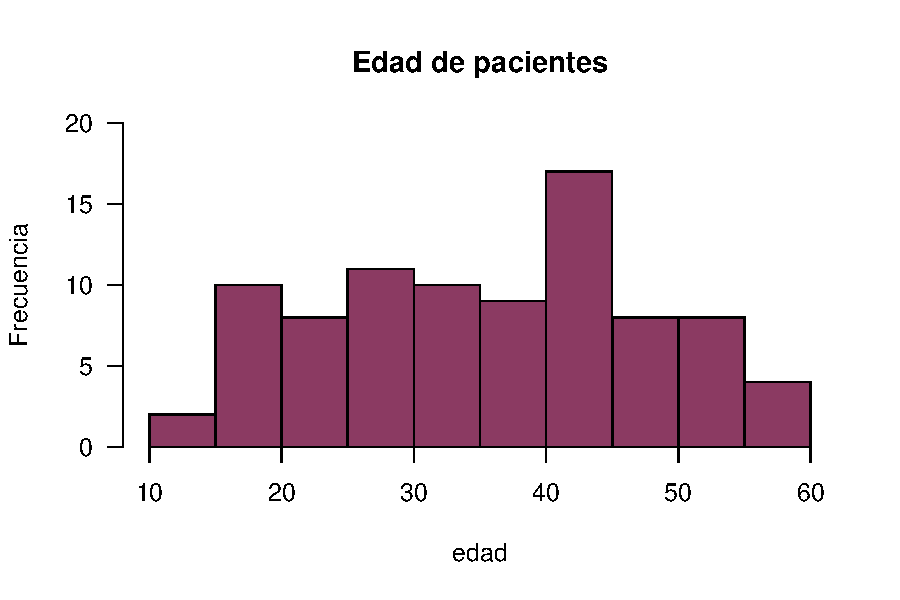
\epsfig{file=EDADES,width=10cm}}	
	 	\caption{\label{fig:prueba} Edad de pacientes.}
	 \end{figure}

	 \begin{figure}[h!tb]        %Poner los ejes de Masculino Femenino
	 	\centerline{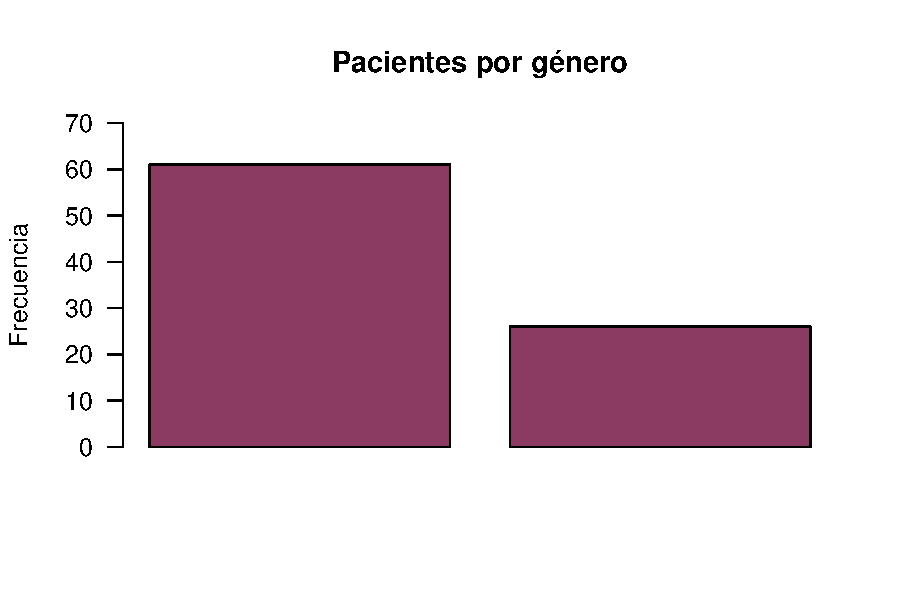
\epsfig{file=GENERO,width=10cm}}	
	 	\caption{\label{fig:prueba} Pacientes por género.}
	 \end{figure}
	 
	\ \\ \ \\ \ \\ 
	En la \textit{Figura 2} se aprecia que la mayoría de los pacientes están en un rango de edad de los 40 a los 45 años, mientras que en el rango de edad con menor incidencia es de los 10 a los 15 años.
	
	La \textit{Figura 3} muestra la frecuencia de desgarre por género. %AQUI NO SE, O SEA SON MÁS H O MÁS M? HAY ALGUNA RAZON?
	%The cause of a hip labral tear may be:
	%   Trauma. Injury to or dislocation of the hip joint — which can occur during car accidents or from playing contact sports such as football or hockey — can cause a hip labral tear.
	%   Structural abnormalities. Some people are born with hip problems that can accelerate wear and tear of the joint and eventually cause a hip labral tear.
	%	Repetitive motions. Sports-related and other physical activities — including the sudden twisting or pivoting motions common in golf or softball — can lead to joint wear and tear that ultimately results in a hip labral tear.
	
	 %vemos que la mayoría de las heridas se encuentran en los pacientes que se con edades entre los 40 y 45 años de edad, mientras que entre los 10 y 15 años es donde menos ocurrencia hay. En la \textit{Figura 3} se aprecia que \textit{columna izquierda} son los(as) que tienen lesiones con más frecuencia. %BUSCAR SI EXISTE UNA RAZÓN MÉDICA PARA ESTO
	 
	 
	 
	
	\ \\
	
	
	
	
	
	
\section{Análisis descriptivo y \textit{aquí poner algo pero no sé qué}}
	En los siguentes conjuntos de gráficas se muestran los resultados de los diagnósticos hechos por cada médico con ambas mediciones, y se compararán entre ellas y con el diagnóstico del cirujano después de hbaer realizasdo la intervención quirúrgica. 
	
%	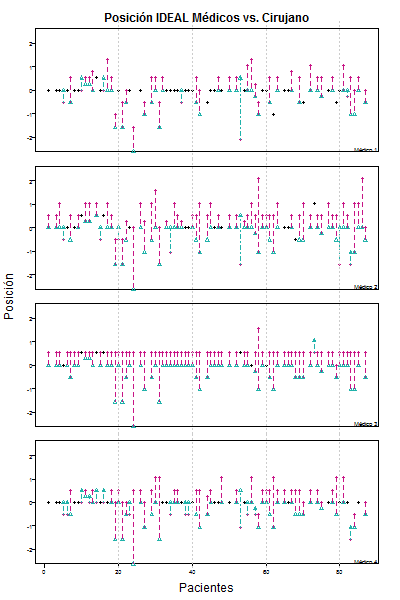
\includegraphics{PosIDEALvsCir}
	\begin{figure}[h!tb]
		\centerline{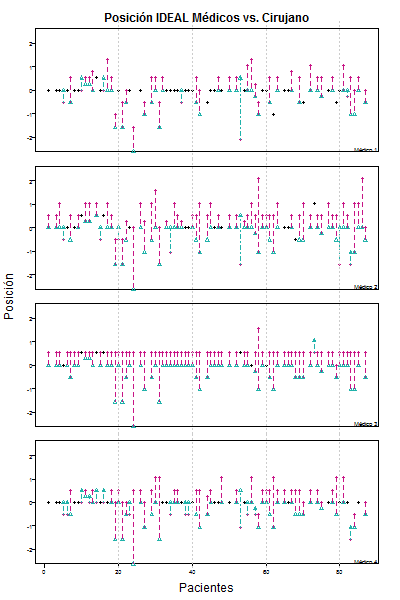
\epsfig{file=PosIDEALvsCir, width=12cm}}
		\caption{\label{fig:prueba} Ideal: círculos rosas. Cirujano: triángulos verdes. Coincide: puntos negros}  %esto suena mal
	\end{figure}			

	\begin{figure}[h!tb]
		\centerline{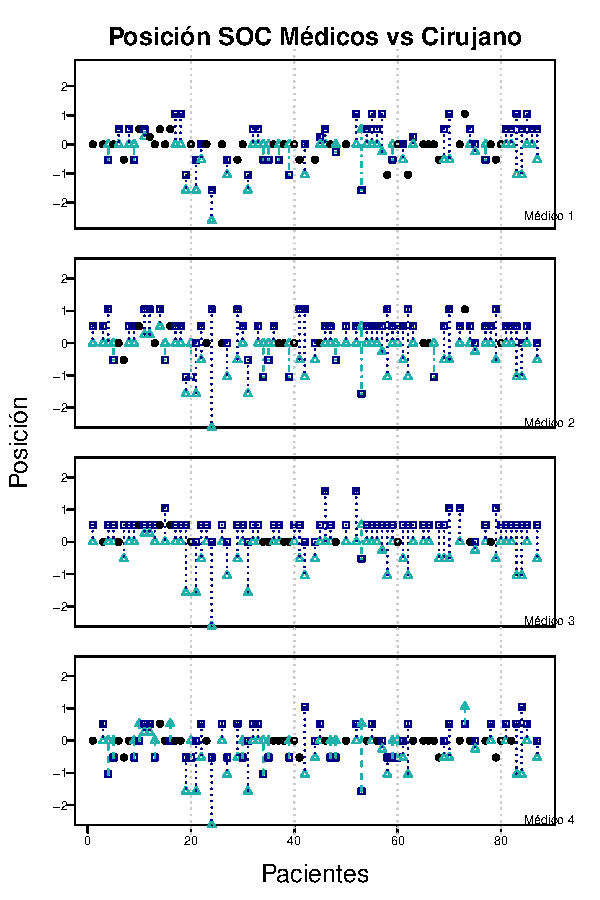
\epsfig{file=PosSOCvsCir, width=12cm}}
		\caption{\label{fig:prueba} SOC vs Cirujano}
	\end{figure}
	
	\begin{figure}[h!tb]
		\centerline{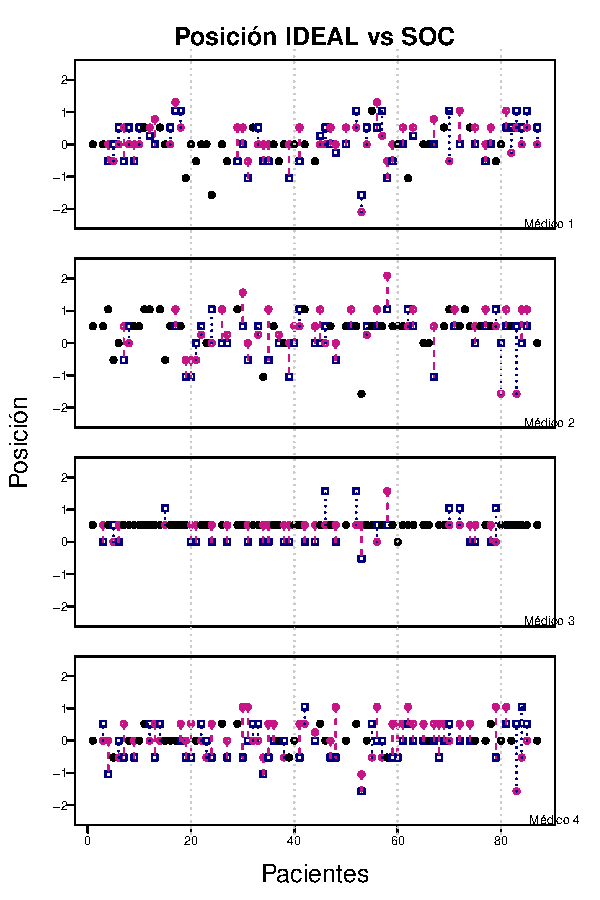
\epsfig{file=PosIDEALvsSOC, width=12cm}}
		\caption{\label{fig:prueba} IDEAL vs SOC}
	\end{figure}
	
	\ \\
	Interpretación de las gráficas: \ \\
	La \textit{Figura 4} corresponde a las gráficas donde se compara la medición de la posición de los cuatro médicos contra el cirujano, para cada uno de los 87 pacientes. Facilmente se observa que la medición realizada por los cutro médicos sobre estima el diagnóstico dinal del cirujano. Por esto podemos concluir que el método Ideal tiende a sobre estimar la medida, es decir, señala que la herida empieza en un punto más alejado positivamente de donde realmente se encuentra.
	
	La \textit{Figura 5} es similar a al anterior, con la diferencai de que muestra el método SOC contra el cirujano. Al igual que el método Ideal, SOC sobre estima la posición real de la herida.
	
	Para comparar cuál de los dos métodos sobre estima más que el otro, se analiza la \textit{Figura 6}. \textsc{No es tan claro, pero parece que Ideal sobre estoma aún más que SOC.}
	
	\end{document}